\documentclass[11pt]{article}
\usepackage[utf8]{inputenc}
\usepackage{amsmath,amssymb}
\usepackage{geometry}
\usepackage{tikz}
\usepackage{listings}
\usepackage{xcolor}
\usepackage{booktabs}
\usepackage{enumitem}
\usepackage{float}
\usepackage[colorlinks=true, linkcolor=blue!70!black, citecolor=green!50!black, urlcolor=blue!60!black]{hyperref}
\usepackage{cleveref}

\usetikzlibrary{calc, angles, quotes, patterns, arrows.meta, decorations.markings, positioning}

\geometry{letterpaper, margin=1in}

% ── Code listing style ───────────────────────────────────────────────
\definecolor{codebg}{rgb}{0.95, 0.95, 0.95}
\definecolor{codegray}{rgb}{0.4, 0.4, 0.4}
\definecolor{codepurple}{rgb}{0.58, 0.0, 0.82}
\definecolor{codeblue}{rgb}{0.13, 0.13, 1}
\definecolor{codegreen}{rgb}{0.0, 0.5, 0.0}

\lstdefinelanguage{JavaScript}{
  keywords={break, case, catch, continue, debugger, default, delete, do, else,
            false, finally, for, function, if, in, instanceof, new, null, return,
            switch, this, throw, true, try, typeof, var, void, while, with,
            let, const},
  morecomment=[l]{//},
  morecomment=[s]{/*}{*/},
  morestring=[b]',
  morestring=[b]",
  keywordstyle=\color{codeblue}\bfseries,
  identifierstyle=\color{black},
  commentstyle=\color{codegreen}\ttfamily,
  stringstyle=\color{codepurple}\ttfamily,
  sensitive=true
}

\lstset{
  language=JavaScript,
  backgroundcolor=\color{codebg},
  basicstyle=\footnotesize\ttfamily,
  showstringspaces=false,
  numbers=left,
  numberstyle=\tiny\color{codegray},
  numbersep=9pt,
  tabsize=2,
  breaklines=true,
  captionpos=b,
  frame=single,
  rulecolor=\color{codegray!40}
}

% ── Shortcuts ─────────────────────────────────────────────────────────
\newcommand{\code}[1]{\texttt{#1}}
\newcommand{\file}[1]{\texttt{#1}}
\newcommand{\key}[1]{\textsf{\textbf{#1}}}

\title{\textbf{ISSF Pistol Sighting Simulator}\\[4pt]
       \large Mathematical Foundation, Physics Reference, and User Guide}
\author{Documentation for \texttt{simulator.js} / \texttt{index.html}}
\date{June 2026}

% ══════════════════════════════════════════════════════════════════════
\begin{document}
\maketitle
\tableofcontents
\clearpage

% ══════════════════════════════════════════════════════════════════════
\section{Introduction}\label{sec:intro}
% ══════════════════════════════════════════════════════════════════════

The ISSF Pistol Sighting Simulator is a browser-based pedagogical tool
that models the optics and physics of \emph{open-sight} (notch-and-post)
pistol marksmanship, shot one-handed and unsupported (free arm).  Unlike
the rifle, whose closed aperture (diopter) sight is treated in the
companion ISSF Rifle Sighting Simulator, the pistol sight picture is a
three-element alignment: the shooter's eye, the rear-sight notch, and the
front post, held against the target~\cite{issf,nra}.

The simulator lets students and athletes isolate, vary, and observe the
effects that are difficult to separate on the range:

\begin{enumerate}[nosep]
  \item \textbf{Sight-alignment (angular) error}---how a small
        displacement of the front post within the rear notch is amplified
        into a large miss downrange (\cref{sec:align}).
  \item \textbf{Arm sway (wobble)}---why a \emph{parallel} movement of the
        whole pistol hurts far less than a constant alignment error
        (\cref{sec:wobble}).
  \item \textbf{Visual accommodation}---why the eye can focus on only one
        plane and must focus on the front sight (\cref{sec:focus}).
  \item \textbf{Hold}---the six-o'clock (sub-six) hold versus the centre
        hold (\cref{sec:hold}).
  \item \textbf{Mechanical sight adjustment}---how rear-sight clicks
        translate into impact shifts (\cref{sec:clicks}).
  \item \textbf{Exterior effects}---gravity, cant, and wind
        (\cref{sec:exterior}).
\end{enumerate}

\noindent Each phenomenon is developed in its own section with the
competitive-shooting context, a physical explanation, a mathematical
derivation, a reference to the implementing JavaScript code, and
suggested exercises with the simulator.

% ══════════════════════════════════════════════════════════════════════
\section{User Manual}\label{sec:manual}
% ══════════════════════════════════════════════════════════════════════

\subsection{Running the Simulator}

Open \file{index.html} in any modern web browser. No build step or
dependency is required; all logic lives in \file{simulator.js} and runs
client-side on an HTML5 canvas. On \href{https://www.tireur.org}{tireur.org}
the simulator is embedded through a PHP wrapper that supplies the same
control panel and loads \file{simulator.js}.

\subsection{Interface Layout}\label{sec:layout}

The canvas is split into two viewports:

\begin{itemize}[nosep]
  \item \textbf{Left --- sight picture.}  The shooter's view of the rear
        notch, the front post, and the target.  A CSS blur is applied per
        plane to simulate visual accommodation (\cref{sec:focus}).
  \item \textbf{Right --- target face.}  The scoring rings, the aiming
        mark, and the predicted/served shots.
\end{itemize}

\noindent Below the canvas, control panels expose the target and aiming
zone, the wobble and wind, the sight alignment, and the mechanical
adjustments, together with a shot table and session statistics (average,
last shot, dispersion).

\subsection{Controls Reference}\label{sec:controls}

The on-screen panels drive the simulator.  When the canvas has focus
(mouse over it), the following keyboard shortcuts are also available:

\begin{center}
\begin{tabular}{ll}
\toprule
\textbf{Input} & \textbf{Action}\\
\midrule
\key{A} / \key{D} & Horizontal alignment error $\mp/\pm 0.02$~mm (0.05 with \key{Shift})\\
\key{W} / \key{S} & Vertical alignment error $\mp/\pm 0.02$~mm\\
\key{Z} / \key{X} & Firearm cant $\mp/\pm 0.5^\circ$\\
\key{Space} & Fire a shot\\
\key{R} & Reset the sights\\
\bottomrule
\end{tabular}
\end{center}

\subsection{Quick-Start Walkthrough}\label{sec:quickstart}

\begin{enumerate}[nosep]
  \item Open the simulator; the default view is a 10\,m air-pistol sight
        picture with the sights perfectly aligned.
  \item Set the focus to \emph{Target sharp, sights blurred} and note how
        alignment becomes impossible to judge---the classic beginner error.
  \item Introduce a small alignment error (\key{A}/\key{D}) and fire
        (\key{Space}); observe how the error is amplified on the card.
  \item Compare with wobble alone (preset \emph{Confirmed}, sights aligned):
        the impact stays much closer to centre.
  \item Switch to the 25\,m target and raise the wind to see the drift grow.
\end{enumerate}

% ══════════════════════════════════════════════════════════════════════
\section{Sight-Alignment (Angular) Error}\label{sec:align}
% ══════════════════════════════════════════════════════════════════════

\subsection{The Issue for Competitive Shooters}

On an open-sight pistol the shooter aligns the front post inside the rear
notch (equal light on either side, tops level) and holds that assembly on
the target.  A small lateral or vertical displacement of the post within
the notch is a tiny angular error of the wrist---but, projected to the
target, it becomes a large miss.

\subsection{Why It Matters}

Sight alignment dominates pistol accuracy because the \emph{sight radius}
$b$ (the distance between the rear notch and the front post) is short
compared with the range $D$.  The lever arm $D/b$ multiplies every
alignment error.  This is the single most important reason a pistol is
harder to shoot than a rifle of equal intrinsic precision~\cite{nra}.

\subsection{Physical Explanation and Illustration}

\Cref{fig:align} shows the geometry.  An offset $e$ of the front post
relative to the line through the eye and the rear notch subtends an angle
$\theta \approx e/b$.  The same angle, carried to the target at range
$D$, produces a displacement
\[
  \Delta \;=\; D\,\tan\theta \;\approx\; \frac{D}{b}\,e .
\]

\begin{figure}[H]
\centering
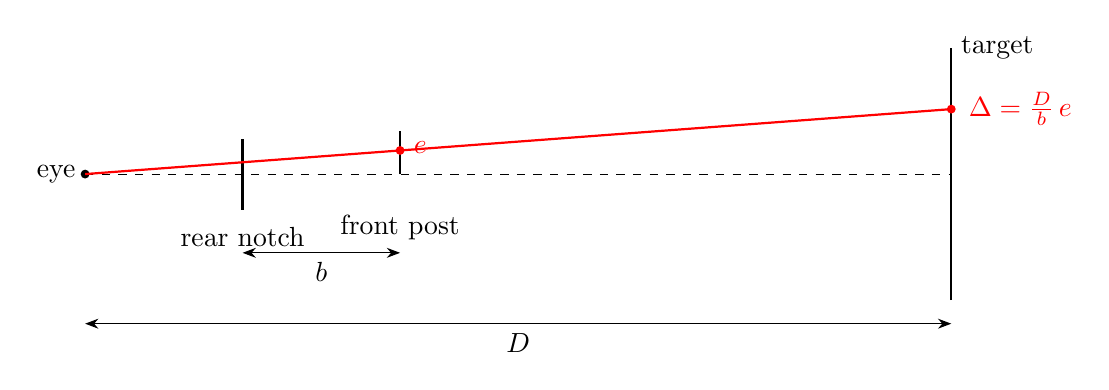
\begin{tikzpicture}[>=Stealth, scale=1.0]
  % baseline (line of sight)
  \draw[dashed] (0,0) -- (11,0);
  % eye
  \fill (0,0) circle (1.6pt);
  \node[left] at (0,0) {eye};
  % rear notch
  \draw[thick] (2,-0.45) -- (2,0.45);
  \node[below] at (2,-0.55) {rear notch};
  % front post (correct, on axis) and offset post
  \draw[thick] (4,0) -- (4,0.55);
  \node[below=10pt] at (4,-0.05) {front post};
  \fill[red] (4,0.30) circle (1.6pt);          % offset post position e
  \node[red, right] at (4.05,0.34) {$e$};
  % target plane
  \draw[thick] (11,-1.6) -- (11,1.6);
  \node[right] at (11,1.6) {target};
  % sight radius brace
  \draw[<->] (2,-1.0) -- (4,-1.0);
  \node[below] at (3,-1.0) {$b$};
  % range brace
  \draw[<->] (0,-1.9) -- (11,-1.9);
  \node[below] at (5.5,-1.9) {$D$};
  % amplified ray
  \draw[red, thick] (0,0) -- (4,0.30) -- (11,0.825);
  \fill[red] (11,0.825) circle (1.6pt);
  \node[red, right] at (11.1,0.825) {$\Delta = \tfrac{D}{b}\,e$};
\end{tikzpicture}
\caption{Sight-alignment error. A front-post offset $e$ over the short
sight radius $b$ is amplified to $\Delta \approx (D/b)\,e$ at the target.}
\label{fig:align}
\end{figure}

\subsection{Mathematical Model}

With sight radius $b$ and range $D$, a small-angle approximation gives the
target displacement from an alignment error $\mathbf{e}=(e_x,e_y)$:
\begin{equation}
  \Delta_x \;=\; \frac{D}{b}\,e_x, \qquad
  \Delta_y \;=\; \frac{D}{b}\,e_y .
  \label{eq:align}
\end{equation}
For the defaults $b = 220$~mm and $D = 10\,000$~mm, the gain is
$D/b \approx 45.5$: an alignment error of only $0.1$~mm becomes
$\approx 4.5$~mm on the card.  At $D=25\,000$~mm the same $0.1$~mm becomes
$\approx 11.4$~mm.

\subsection{Implementation}

\begin{lstlisting}
const distScale = activeTarget.distance_mm / L_SIIGHT_RADIUS_MM; // D / b
const alignmentShiftX = alignErrX * distScale;
const alignmentShiftY = alignErrY * distScale;
\end{lstlisting}

The alignment vector is then rotated by the cant angle (\cref{sec:exterior})
before being added to the impact point.

\subsection{Simulator Exercises}

\begin{enumerate}[nosep]
  \item Set the alignment error to $0.1$~mm horizontally and read the
        target shift; verify it matches $D/b \times 0.1$~mm.
  \item Switch from 10\,m to 25\,m and confirm the same alignment error
        now costs more than twice as many millimetres.
\end{enumerate}

% ══════════════════════════════════════════════════════════════════════
\section{Arm Sway (Wobble): Angular vs.\ Parallel Error}\label{sec:wobble}
% ══════════════════════════════════════════════════════════════════════

\subsection{The Issue for Competitive Shooters}

Held at arm's length with one hand, the pistol never stops moving.  This
\emph{wobble area} is a \emph{parallel} displacement of the whole sight
system relative to the target: the sights stay aligned, but the aligned
assembly drifts over the aiming mark.

\subsection{Why It Matters}

A parallel error maps \emph{one-to-one} onto the target (gain $1$), whereas
an alignment error is amplified by $D/b$ (\cref{eq:align}).  Hence the
classic coaching rule: it is better to release a shot with a small wobble
and perfect sight alignment than with the gun frozen on centre but the
sights misaligned~\cite{nra}.

\subsection{Physical Explanation and Illustration}

\Cref{fig:angvspar} contrasts the two errors.  An alignment error is taken
over the short sight radius and amplified by $D/b$, while a parallel wobble
of the correctly aligned assembly is carried to the target unchanged.

\begin{figure}[H]
\centering
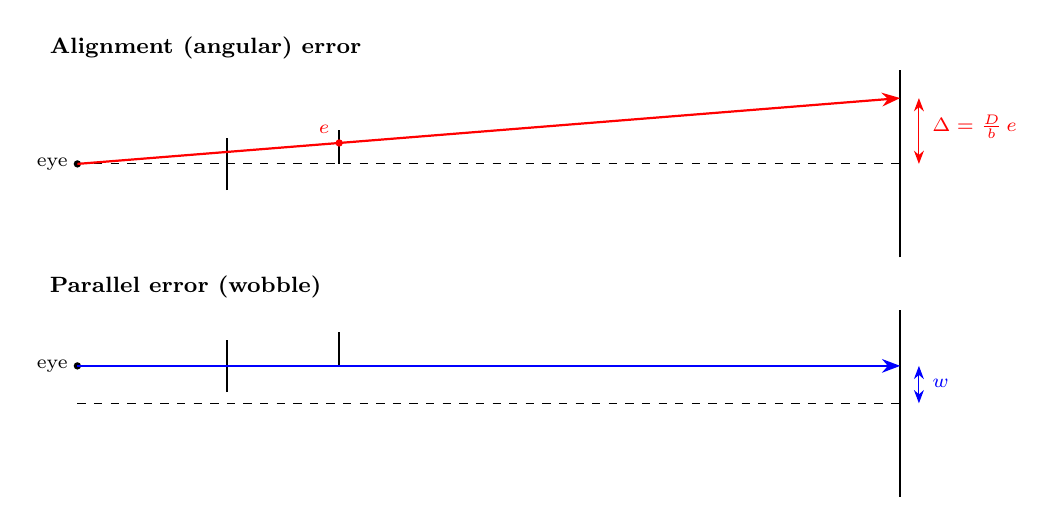
\begin{tikzpicture}[>=Stealth, scale=0.95]
  % ---- Top: angular (alignment) error ----
  \begin{scope}
    \node[anchor=west] at (-0.5,1.55) {\footnotesize\textbf{Alignment (angular) error}};
    \draw[dashed] (0,0) -- (11,0);
    \fill (0,0) circle (1.4pt); \node[left] at (0,0) {\scriptsize eye};
    \draw[thick] (2,-0.35) -- (2,0.35);
    \draw[thick] (3.5,0) -- (3.5,0.45);
    \fill[red] (3.5,0.28) circle (1.4pt);
    \node[red, above left] at (3.5,0.28) {\scriptsize $e$};
    \draw[thick] (11,-1.25) -- (11,1.25);
    \draw[red, thick, ->] (0,0) -- (3.5,0.28) -- (11,0.88);
    \draw[red, <->] (11.25,0) -- (11.25,0.88);
    \node[red, right] at (11.3,0.5) {\scriptsize $\Delta=\frac{D}{b}\,e$};
  \end{scope}
  % ---- Bottom: parallel (wobble) error ----
  \begin{scope}[yshift=-3.2cm]
    \node[anchor=west] at (-0.5,1.55) {\footnotesize\textbf{Parallel error (wobble)}};
    \draw[dashed] (0,0) -- (11,0);
    \fill (0,0.5) circle (1.4pt); \node[left] at (0,0.5) {\scriptsize eye};
    \draw[thick] (2,0.15) -- (2,0.85);
    \draw[thick] (3.5,0.5) -- (3.5,0.95);
    \draw[thick] (11,-1.25) -- (11,1.25);
    \draw[blue, thick, ->] (0,0.5) -- (11,0.5);
    \draw[blue, <->] (11.25,0) -- (11.25,0.5);
    \node[blue, right] at (11.3,0.27) {\scriptsize $w$};
  \end{scope}
\end{tikzpicture}
\caption{Angular vs.\ parallel error (schematic, not to scale). A front-post
offset $e$ is amplified to $\Delta=(D/b)\,e$ (top); a parallel wobble $w$ of
the aligned assembly maps one-to-one to the target (bottom).}
\label{fig:angvspar}
\end{figure}

\subsection{Mathematical Model}

The wobble is modelled as a quasi-periodic sum of sinusoids with amplitude
set by the stability preset.  Writing $A$ for the preset scale, the
displacement is
\begin{align}
  w_x(t) &= 2A\big[0.60\sin(1.1\,t) + 0.35\sin(0.35\,t) + 0.05\cos(2.1\,t)\big],\\
  w_y(t) &= 2A\big[0.50\cos(0.9\,t) + 0.40\sin(0.45\,t) + 0.10\sin(1.8\,t)\big],
\end{align}
which the aiming point inherits directly, $a_{x,y} = m_{x,y} + w_{x,y}$,
with no $D/b$ amplification. The presets are $A=0$ (bench), $2$ (expert),
$5$ (confirmed), and $10$ (beginner), in millimetre scale.

\subsection{Implementation}

\begin{lstlisting}
const baseAmp = wobbleAmp * 2.0;
wobbleX = baseAmp * (Math.sin(wobbleTime*1.1)*0.6 + Math.sin(wobbleTime*0.35)*0.35 + Math.cos(wobbleTime*2.1)*0.05);
wobbleY = baseAmp * (Math.cos(wobbleTime*0.9)*0.5 + Math.sin(wobbleTime*0.45)*0.4 + Math.sin(wobbleTime*1.8)*0.1);
\end{lstlisting}

\subsection{Simulator Exercises}

\begin{enumerate}[nosep]
  \item With the \emph{Beginner} preset and perfect alignment, fire ten
        shots and note the group size; it reflects the wobble amplitude
        almost directly.
  \item Repeat with a fixed $0.1$~mm alignment error and the \emph{bench}
        preset: the group is tight but badly off-centre---the amplified
        angular error.
\end{enumerate}

% ══════════════════════════════════════════════════════════════════════
\section{Visual Accommodation (Front-Sight Focus)}\label{sec:focus}
% ══════════════════════════════════════════════════════════════════════

\subsection{The Issue for Competitive Shooters}

The eye can sharply focus on only one plane at a time.  Three planes
compete for focus: the rear notch ($\approx 0.5$~m), the front post
($\approx 0.7$~m), and the target ($10$--$25$~m).  Beginners instinctively
focus on the target; experts focus on the \emph{front sight}.

\subsection{Why It Matters}

Sight-alignment error (\cref{sec:align}) can only be judged if the front
post and notch are sharp.  Focusing on the target blurs the sights and
makes alignment guesswork, reintroducing the most heavily amplified error
of all.  A sharp front sight is therefore the prerequisite for everything
else.

\subsection{Physical Explanation}

Depth of field around the focused plane is finite; planes outside it form
a blur circle whose diameter grows with the dioptric distance from focus.
The simulator renders this with a per-plane Gaussian blur (in pixels),
choosing the front-focus profile as the ``correct'' one (\cref{fig:focusfig}):

\begin{figure}[H]
\centering
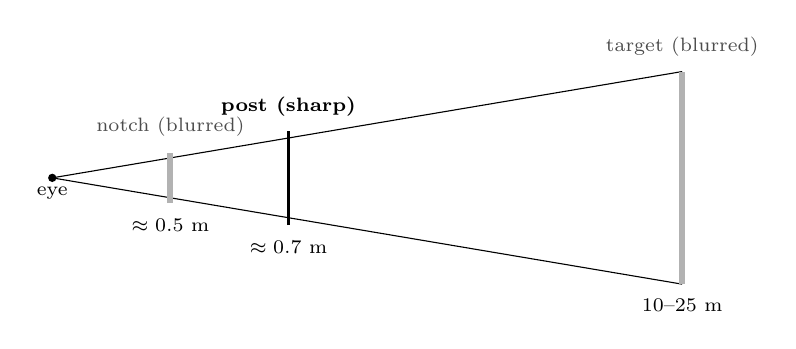
\begin{tikzpicture}[>=Stealth, scale=1.0]
  \fill (0,0) circle (1.5pt); \node[below] at (0,0) {\scriptsize eye};
  % cone of vision
  \draw (0,0) -- (8,1.35); \draw (0,0) -- (8,-1.35);
  % rear notch plane (blurred)
  \draw[gray!60, line width=2.2pt] (1.5,-0.32) -- (1.5,0.32);
  \node[gray!60!black, above] at (1.5,0.4) {\scriptsize notch (blurred)};
  \node[below] at (1.5,-0.4) {\scriptsize $\approx 0.5$ m};
  % front post plane (sharp)
  \draw[black, line width=1pt] (3,-0.6) -- (3,0.6);
  \node[above] at (3,0.66) {\scriptsize \textbf{post (sharp)}};
  \node[below] at (3,-0.68) {\scriptsize $\approx 0.7$ m};
  % target plane (blurred, far)
  \draw[gray!60, line width=2.2pt] (8,-1.35) -- (8,1.35);
  \node[gray!60!black, above] at (8,1.42) {\scriptsize target (blurred)};
  \node[below] at (8,-1.42) {\scriptsize $10$--$25$ m};
\end{tikzpicture}
\caption{Visual accommodation (schematic, not to scale). The eye focuses on a
single plane; the front post is kept sharp while the rear notch and the target
are left blurred.}
\label{fig:focusfig}
\end{figure}

\begin{center}
\begin{tabular}{lccc}
\toprule
\textbf{Focus} & \textbf{Front post} & \textbf{Rear notch} & \textbf{Target}\\
\midrule
Front (correct)   & 0   & 1.5 & 8\\
Target (error)    & 6   & 9   & 0\\
Rear              & 2.5 & 0   & 9\\
\bottomrule
\end{tabular}
\end{center}

\subsection{Implementation}

\begin{lstlisting}
function getBlurFilters() {
  if (focusType === "front")  return { front: 0,   rear: 1.5, target: 8 };
  if (focusType === "target") return { front: 6,   rear: 9,   target: 0 };
  return { front: 2.5, rear: 0, target: 9 }; // rear focus
}
\end{lstlisting}

\subsection{Simulator Exercises}

Cycle through the three focus modes while holding a small alignment error.
Only in front-focus is the misalignment clearly visible---demonstrating why
the front sight must stay sharp.

% ══════════════════════════════════════════════════════════════════════
\section{Hold: Six-O'Clock vs.\ Centre}\label{sec:hold}
% ══════════════════════════════════════════════════════════════════════

\subsection{The Issue for Competitive Shooters}

Two holds are common in precision pistol.  In the \emph{six-o'clock} (or
sub-six) hold the shooter places the front post just under the black bull,
leaving a thin band of white; the sights are zeroed so the bullet still
strikes the centre.  In the \emph{centre} hold the point of aim equals the
point of impact.

\subsection{Why It Matters}

A black front post against a black bull is hard to align precisely.  The
six-o'clock hold detaches the post from the bull against a white
background, sharpening the alignment and elevation judgment.  The trade-off
is sensitivity to changes in light and bull size.

\subsection{Mathematical Model}

The six-o'clock hold offsets the aiming mark below centre by the bull
radius plus a small white margin, $h_{\text{hold}} = r_{\text{black}} + 6$~mm,
and the sight zero adds the same amount back, so a correctly aligned shot
lands at the centre:
\begin{equation}
  m_y^{(0)} = -\,h_{\text{hold}}, \qquad
  \text{zero offset} = +\,h_{\text{hold}} .
\end{equation}

\subsection{Implementation}

\begin{lstlisting}
const holdOffset_zero = (holdType === "6oclock")
                        ? (activeTarget.black_r + 6.0) : 0.0;
// aim point default: mouseAimY = -(black_r + 6.0) for the six-o'clock hold
\end{lstlisting}

% ══════════════════════════════════════════════════════════════════════
\section{Mechanical Sight Adjustment (Clicks)}\label{sec:clicks}
% ══════════════════════════════════════════════════════════════════════

\subsection{The Issue for Competitive Shooters}

The rear sight is adjustable in windage and elevation by detented clicks.
A target-pistol click is typically $0.1$~mrad, moving the zero by a fixed,
range-dependent amount.

\subsection{Mathematical Model}

For an angular click value $\delta = 0.1$~mrad and range $D$, one click
moves the impact by $D\,\delta$:
\begin{equation}
  \Delta_{\text{click}} = D\,\delta \approx
  \begin{cases}
    1.0~\text{mm} & D = 10~\text{m},\\
    2.5~\text{mm} & D = 25~\text{m}.
  \end{cases}
\end{equation}
A positive windage click moves the impact right; a positive elevation
click moves it up.

\subsection{Implementation}

\begin{lstlisting}
const clickX_mm = clicksX * activeTarget.click_value_mm;
const clickY_mm = clicksY * activeTarget.click_value_mm;
\end{lstlisting}

% ══════════════════════════════════════════════════════════════════════
\section{Exterior Effects: Gravity, Cant, and Wind}\label{sec:exterior}
% ══════════════════════════════════════════════════════════════════════

\subsection{Gravity}

The projectile falls under gravity during its time of flight $t = D/v$.
The drop is~\cite{mccoy}
\begin{equation}
  y_{\text{drop}} = \tfrac{1}{2}\,g\,t^2 = \tfrac{1}{2}\,g\left(\frac{D}{v}\right)^2 .
\end{equation}
The sights are zeroed for this drop, so it matters only through the cant
interaction below.  With $v=175$~m/s at 10\,m the drop is a fraction of a
millimetre; with $v=330$~m/s at 25\,m it is a few millimetres.

\subsection{Cant}

Tilting the pistol by an angle $\phi$ about the bore rotates the sight
correction (sight height $h$ plus zeroed drop) out of the vertical,
producing \emph{both} a lateral shift and a vertical loss---the canting
paradox~\cite{rinker}:
\begin{align}
  \Delta x_{\text{cant}} &= (h + y_{\text{drop}})\sin\phi,\\
  \Delta y_{\text{cant}} &= (h + y_{\text{drop}})(1-\cos\phi).
\end{align}
The alignment error vector \eqref{eq:align} is likewise rotated by $\phi$.
\Cref{fig:cantfig} shows how the upright sight-height correction, once
canted, splits into a lateral shift and a vertical loss.

\begin{figure}[H]
\centering
\begin{tikzpicture}[>=Stealth, scale=1.3]
  \def\cantang{25}
  \fill (0,0) circle (1.2pt); \node[below right=1pt] at (0,0) {\scriptsize bore axis};
  % intended (upright) sight-height vector
  \draw[dashed, ->] (0,0) -- (0,2);
  \node[above] at (0,2) {\scriptsize $h$ (upright)};
  % canted vector
  \draw[thick, ->] (0,0) -- ({-2*sin(\cantang)},{2*cos(\cantang)});
  \node[above left] at ({-2*sin(\cantang)},{2*cos(\cantang)}) {\scriptsize $h$ (canted)};
  % cant angle arc + label
  \draw (0,1.3) arc (90:115:1.3);
  \node at (-0.34,1.5) {\scriptsize $\phi$};
  % guides
  \draw[dotted] ({-2*sin(\cantang)},{2*cos(\cantang)}) -- ({-2*sin(\cantang)},0);
  \draw[dotted] ({-2*sin(\cantang)},{2*cos(\cantang)}) -- (2.2,{2*cos(\cantang)});
  \draw[dotted] (0,2) -- (2.2,2);
  % lateral shift
  \draw[red, <->] ({-2*sin(\cantang)},-0.42) -- (0,-0.42);
  \node[red, below] at ({-1*sin(\cantang)},-0.44) {\scriptsize $h\sin\phi$};
  % vertical loss
  \draw[blue, <->] (2.2,{2*cos(\cantang)}) -- (2.2,2);
  \node[blue, right] at (2.25,{cos(\cantang)+1}) {\scriptsize $h(1-\cos\phi)$};
\end{tikzpicture}
\caption{The canting paradox. Tilting the pistol by $\phi$ rotates the upright
sight-height correction $h$, producing both a lateral shift $h\sin\phi$ and a
vertical loss $h(1-\cos\phi)$.}
\label{fig:cantfig}
\end{figure}

\subsection{Wind}

Only the crosswind (lateral) component deflects the bullet appreciably at
pistol ranges.  With wind speed $w$ from clock direction $\varphi$
($\varphi = 90^\circ$ from the right) and a range-dependent factor $k$,
\begin{equation}
  \Delta x_{\text{wind}} = -\,w\,k\,\sin\varphi, \qquad \Delta y_{\text{wind}} = 0,
\end{equation}
with $k = 0.5$~mm/(m/s) at 10\,m and $1.5$~mm/(m/s) at 25\,m.

\subsection{Total Impact}

Collecting all terms, the impact point (mm from centre) is
\begin{align}
  X &= a_x + \Delta_x^{\text{align}} + \Delta x_{\text{cant}} + \Delta x_{\text{wind}} + \Delta_x^{\text{click}},\\
  Y &= a_y + \Delta_y^{\text{align}} - \Delta y_{\text{cant}} + h_{\text{hold}} + \Delta_y^{\text{click}},
\end{align}
where $a_{x,y}$ is the aim point including wobble.

% ══════════════════════════════════════════════════════════════════════
\section{Scoring Model}\label{sec:scoring}
% ══════════════════════════════════════════════════════════════════════

\subsection{ISSF Decimal Scoring}

The score is a function of the radial distance $\rho = \sqrt{X^2+Y^2}$ of
the shot centre from the target centre, interpolated linearly within each
ring so that a decimal value $1.0$--$10.9$ is produced; the innermost zone
is the \emph{inner ten} (``mouche'').  Ring spacing is $8$~mm at 10\,m and
$25$~mm at 25\,m.

\subsection{Implementation}

\begin{lstlisting}
const dist = Math.hypot(x_mm, y_mm);
// 10 m: inner ten within 2.5 mm; rings every 8 mm
const ringIndex = Math.floor((dist - 5.75) / 8.0);
const fraction  = (dist - (5.75 + ringIndex*8.0)) / 8.0;
return { score: Math.max(1.0, 9.9 - ringIndex - fraction), isMouche: false };
\end{lstlisting}

% ══════════════════════════════════════════════════════════════════════
\section{Implementation Notes}\label{sec:implementation}
% ══════════════════════════════════════════════════════════════════════

\subsection{Coordinate System}

All physical quantities are in millimetres on the target plane; the origin
is the target centre, $x$ to the right and $y$ upward.  The left viewport
draws the sight picture at \code{PX\_PER\_MM\_SIGHT = 25} px/mm; the right
viewport draws the target face at the per-target \code{scale\_right}.

\subsection{Physical Constants and Defaults}

\begin{center}
\begin{tabular}{lll}
\toprule
\textbf{Symbol} & \textbf{Code} & \textbf{Default}\\
\midrule
Sight radius $b$ & \code{L\_SIIGHT\_RADIUS\_MM} & 220 mm\\
Sight height $h$ & \code{sightHeightOffset} & 45 mm\\
Click value $\delta$ & \code{click\_value\_mm} & 1.0 / 2.5 mm\\
Wind factor $k$ & \code{wind\_factor} & 0.5 / 1.5 mm/(m/s)\\
Muzzle velocity $v$ & \code{muzzle\_velocity\_mps} & 175 / 330 m/s\\
\bottomrule
\end{tabular}
\end{center}

\noindent The identifier \code{L\_SIIGHT\_RADIUS\_MM} retains its original
(misspelled) spelling from the source for fidelity to the code.

% ══════════════════════════════════════════════════════════════════════
\begin{thebibliography}{9}

\bibitem{issf}
  International Shooting Sport Federation,
  \textit{ISSF Official Statutes, Rules and Regulations},
  ISSF, 2024 edition.

\bibitem{nra}
  National Rifle Association,
  \textit{NRA Guide to Pistol Marksmanship},
  NRA Publications, 2014.

\bibitem{mccoy}
  R.\,L.~McCoy,
  \textit{Modern Exterior Ballistics},
  2nd ed.\@ Schiffer Publishing, 2012.
  ISBN 978-0-7643-3825-0.

\bibitem{rinker}
  R.\,A.~Rinker,
  \textit{Understanding Firearm Ballistics},
  6th ed.\@ Mulberry House Publishing, 2005.
  ISBN 978-0-9645598-3-4.

\end{thebibliography}

\end{document}
